\documentclass{standalone}
\usepackage{tikz}
\usepackage{verbatim}
\usetikzlibrary{positioning}
\begin{document}
\pagestyle{empty}
  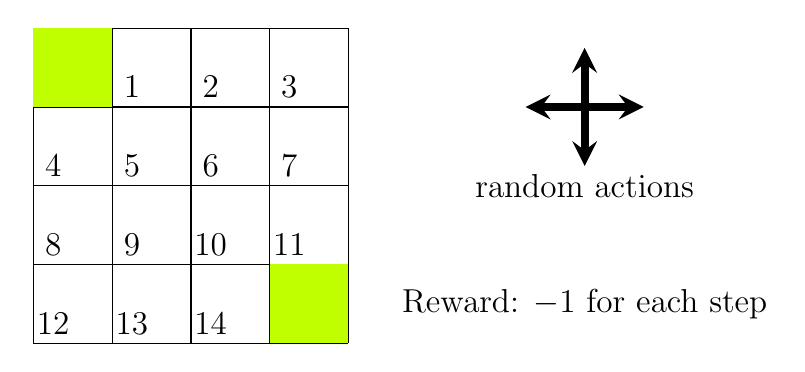
\begin{tikzpicture}
    \draw[stealth-stealth, line width=1 mm] (7.75, 3) -- (6.25, 3);
    \draw[stealth-stealth, line width=1 mm] (7, 2.25) -- (7, 3.75);
    \node at (7, 2) {\large random actions};
    \node at (7, 0.5) {\large Reward: $-1$ for each step};
    \draw[step=1.0,black] (0,0) grid (4, 4);
    \fill[lime] (0, 3) rectangle (1,4);
    \fill[lime] (3, 0) rectangle (4,1);
    % Top row.
    \node at (1.25, 3.25) {\large 1};
    \node at (2.25, 3.25) {\large 2};
    \node at (3.25, 3.25) {\large 3};
    % Second frop top row.
    \node at (0.25, 2.25) {\large 4};
    \node at (1.25, 2.25) {\large 5};
    \node at (2.25, 2.25) {\large 6};
    \node at (3.25, 2.25) {\large 7};
    % Second from bottom row.
    \node at (0.25, 1.25) {\large 8};
    \node at (1.25, 1.25) {\large 9};
    \node at (2.25, 1.25) {\large 10};
    \node at (3.25, 1.25) {\large 11};
    % Bottom row.
    \node at (0.25, 0.25) {\large 12};
    \node at (1.25, 0.25) {\large 13};
    \node at (2.25, 0.25) {\large 14};
    
  \end{tikzpicture}
\end{document}